\documentclass[dvipdfmx,a4j,11pt]{jarticle}
%\usepackage[a4paper,text={17cm,25cm},centering]{geometry}	% to expand the text area
\usepackage{graphicx}
\usepackage{amssymb}
\usepackage{epstopdf}
\DeclareGraphicsRule{.tif}{png}{.png}{`convert #1 `dirname #1`/`basename #1 .tif`.png}
\usepackage{ascmac}
\usepackage{multicol}
\usepackage{udline}
\usepackage{bm}
\usepackage{qexam}

\newenvironment{inputbox}{%
	\begin{itembox}[r]{\LaTeX ソース}
}{
	\end{itembox}
}

\newenvironment{outputbox}{%
	\begin{itembox}[r]{出力}
}{%
	\end{itembox}
}

\addtolength{\questionTopMargin}{-5mm}
\addtolength{\questionBottomMargin}{-5mm}
\addtolength{\qlistTopMargin}{-7mm}
\addtolength{\qlistBottomMargin}{-7mm}

\title{{\bf qexam.sty} v2.1\\
試験問題用\LaTeX スタイルファイル}
\author{山中 卓\\
{\tt taku@hep.sci.osaka-u.ac.jp}\\
大阪大学大学院理学研究科 物理学専攻}
\date{2020年8月15日}                                           % Activate to display a given date or no date

\begin{document}
\西暦
\maketitle
\begin{abstract}
	\texttt{qexam.sty} は、試験問題を作るときのための\LaTeX スタイルファイルです。
	これにより、大門、中問、小問を論理的に構成して書くことができます。
	また、中問を横断して連続した番号のついた小問を並べられます。
	番号の割り振りは\LaTeX の{\tt enumerate}環境のように自動的に行われるので、楽で安全です。
\end{abstract}

改定履歴
\begin{itemize}
	\item [v2.1:] 2020-08-15
		\begin{itemize}
			\item qparts をitemizeではなく、listに変更し、\textbackslash qpart
				内での段落が字下げされるようにした。
			\item \textbackslash arabicz に未定義のreferenceが来た場合でも
				エラーとならないようにした。
		\end{itemize}
		
	\item [v2.0:] 2019-06-18
		\begin{itemize}
			\item 書式をよりカスタマイズできるようにした。
			\item 湯川諭氏の手法を取り入れ、全角の問題番号もサポートした。
			\item 穴埋め式問題用の箱(\textbackslash qbox)を追加。
		\end{itemize}
	\item[v1.3:] 2009-07-11.\\
			 qexam.styをいじらずに、様々なカスタマイズができるようにした。\\
			 geometryやpagestyle\{empty\}等の設定はユーザーのファイルの中で行うようにした。
\end{itemize}

\clearpage
\tableofcontents
\clearpage
%\section{はじめに}
%\texttt{qexam.sty} は、試験問題を作るときのための\LaTeX スタイルファイルです。
%これにより、大門、中問、小問を論理的に構成して書くことができます。
%また、中問を横断して連続した番号のついた小問を並べられます。
%番号の割り振りは\LaTeX の{\tt enumerate}環境のように自動的に行われるので、楽で安全です。

\section{{\tt qexam.sty}関係のファイル}
	次のファイルが付属されています。
	\begin{itemize}
		\item {\tt qexam.sty}: 試験問題作成用のスタイルファイル
		\item {\tt qexam\_doc.pdf}: このマニュアル
		\item {\tt qexam\_examples.tex}: 試験問題の例
		\item {\tt qexam\_template.tex}: ひな形
	\end{itemize}
	
	このマニュアルを読むのが面倒な方は、{\tt qexam\_examples.tex}をタイプセットして、
	ソースと出力を見比べてください。
	
\section{使い方}
\subsection{{\bf qexam}パッケージを読み込む}
	まず、{\tt qexam.sty}のファイルを、\LaTeX のソースファイルと同じdirectoryにコピーします。
	
	次に\LaTeX のソースファイルの頭に、次の1行を入れます。
	\begin{inputbox}
		\begin{verbatim}
			\usepackage{qexam}
		\end{verbatim}
	\end{inputbox}
	
		
\subsection{大問}
	大問の開始は
	{\tt \verb"\question{...}"}を用いて、問題番号(名前)を指定します。
	2番目以降の大問の場合は、この直前に
%	\begin{verbatim}
		\verb"\clearpage"
%	\end{verbatim}
	を入れて改ページする事が多いでしょう。
	\begin{inputbox}
		\begin{verbatim}
			\clearpage
			\question{問題1}
		\end{verbatim}
	\end{inputbox}
	
%	\begin{outputbox}
%		\question{問題1}
%	\end{outputbox}
	
	
\subsection{小問}
	 小問は、次のように{\tt qlist}環境でくくり、
	 各小問は{\tt \textbackslash qitem}で始めます。

	 \begin{inputbox}
		\begin{verbatim}
			\begin{qlist}
		    \qitem 謎の物体$X$の正体を明かせ。
		    \qitem \label{q:Xforce} 謎の物体$X$にかかる力を求めよ。
		    \qitem 小問\qref{q:Xforce}の結果を用い、謎の物体$X$の軌道を求めよ。
			\end{qlist}
		\end{verbatim}
	\end{inputbox}
	
	\begin{outputbox}
		\begin{qlist}
		    \qitem 謎の物体$X$の正体を明かせ。
		    \qitem \label{q:Xforce} 謎の物体$X$にかかる力を求めよ。
		    \qitem 小問\qref{q:Xforce}の結果を用い、謎の物体$X$の軌道を求めよ。
		\end{qlist}
	\end{outputbox}
	
\subsection{小問の参照}
	小問にはラベルを割り振って、他から参照する事もできます。
	上の例のように、ラベルは通常通り{\tt \textbackslash label\{...\}}でつけます。
	参照する場合は、
	{\tt \textbackslash qref\{...\}}を用います。
	({\tt \textbackslash ref\{...\}}だと、小問の番号に( )が付きません。)
	
\subsection{小問の中の問題(微小問?)}
	小問の中にさらに問題を並べるには、{\tt qlist2}環境を用います。
	
	\begin{inputbox}
		\begin{verbatim}
			\begin{qlist}
			    \qitem ジェダイの力によって宇宙のダークマターが一掃された場合の影響について述べよ。
			    \qitem 次の物の違いを述べよ。
			        \begin{qlist2}
			            \qitem ダークエネルギーとダークフォース
			            \qitem ダークマターとダークダックス
			        \end{qlist2}
			        
			\end{qlist}
		\end{verbatim}
	\end{inputbox}
	
	\begin{outputbox}
			\begin{qlist}
			    \qitem ジェダイの力によって宇宙のダークマターが一掃された場合の影響について述べよ。
			    \qitem 次の物の違いを述べよ。
			        \begin{qlist2}
			            \qitem ダークエネルギーとダークフォース
			            \qitem ダークマターとダークダックス
			        \end{qlist2}
			        
			\end{qlist}
	\end{outputbox}
	
\subsection{中問}
	問題の中で、異なる条件をいくつか設定する場合には、
	条件ごとに中問を作り、小問をまとめた方が分かりやすくなります。
	もし中問がある場合は、{\tt qparts}環境でくくり、中に{\tt \textbackslash qpart}を用いて中問を並べます。
	中問には、{\bf I}, {\bf II}, {\bf III}, ...のようにローマ数字の問題番号が割り振られます。
	
	中問ごとに{\tt qlist}環境を作り、小問を並べます。
	小問の番号(1), (2), ...は、中問が変わっても連続した数が割り振られます。
	
	\begin{inputbox}
		\begin{verbatim}
			\begin{qparts}
			    \qpart まず、フォースが働かない場合を考えよう。
			        \begin{qlist}
			            \qitem Yodaにかかる力を図示せよ。
			            \qitem Lukeが宇宙船に及ぼせる力の上限を求めよ。
			        \end{qlist}
			        
			    \qpart 次に、フォースが働く場合を考えよう。
			        \begin{qlist}
			            \qitem \label{q:forcerange}
			                  フォースの距離依存性を式で表せ。
			            \qitem Lukeが宇宙船を持ち上げられるか、
			                    \qref{q:forcerange}の結果を元に計算して求めよ。
			        \end{qlist}
			\end{qparts}
		\end{verbatim}
	\end{inputbox}
	
	\setcounter{qpartNumber}{0}	% reset counter for this document
	\setcounter{enumqSave}{0}
	
	\begin{outputbox}
			\begin{qparts}
			    \qpart まず、フォースが働かない場合を考えよう。
			        \begin{qlist}
			            \qitem Yodaにかかる力を図示せよ。
			            \qitem Lukeが宇宙船に及ぼせる力の上限を求めよ。
			        \end{qlist}
			        
			    \qpart 次に、フォースが働く場合を考えよう。
			        \begin{qlist}
			            \qitem \label{q:forcerange}
			                  フォースの距離依存性を式で表せ。
			            \qitem Lukeが宇宙船を持ち上げられるか、
			                    \qref{q:forcerange}の結果を元に計算して求めよ。
			        \end{qlist}
			\end{qparts}

	\end{outputbox}

\subsection{穴埋め問題}
	穴埋め問題も、\verb"\qbox{}"を用いて作れます。
	\verb"\qbox{}" というように引数を空にすると、自動的に増える番号が箱の中に入ります。
	\verb"\qbox{(99)}"というように引数を与えると、その引数がそのまま箱の中に入ります。
	\begin{inputbox}
		\begin{verbatim}
			次の文章の \qbox{(a)}から\ \qbox{(b)} にあてはまる言葉を書け。\\
        		
			\qbox{}を持つことができるのはジェダイだけである。
			それが暗くなると\qbox{}になるが、発音を間違えるとダークホースになるので注意が必要である。
		\end{verbatim}
	\end{inputbox}
	
	\begin{outputbox}
		次の文章の \qbox{(a)}から\ \qbox{(b)} にあてはまる言葉を書け。\\
		
		\qbox{}を持つことができるのはジェダイだけである。
		それが暗くなると\qbox{}になるが、発音を間違えるとダークホースになるので注意が必要である。
	\end{outputbox}

\subsection{図や表のキャプション}
	通常、図や表のキャプションは「図1: ...」のように、図の番号の後にコロン (:)が付きます。
	キャプションの文章が入らない場合このコロンは邪魔であるため、
	{\tt qexam.sty}ではコロンを出力しないようにしています。
	\begin{inputbox}
		\begin{verbatim}
		\begin{figure}[htbp]
		    \begin{center}
		        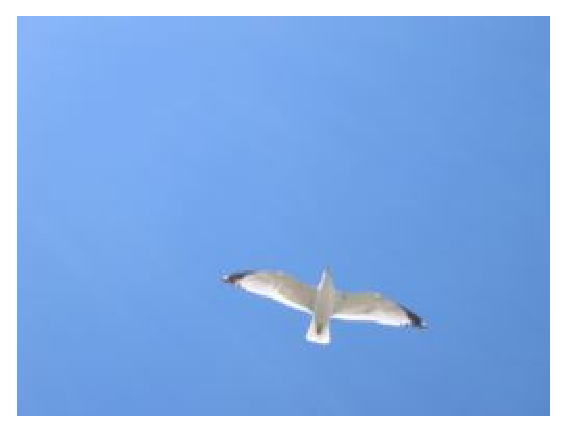
\includegraphics[width=0.4\linewidth]{seagull2.eps}
		        \caption{\label{fig:seagull}}
		    \end{center}
		\end{figure}
		\end{verbatim}
	\end{inputbox}
	
		\begin{figure}[htbp]
			\begin{center}
				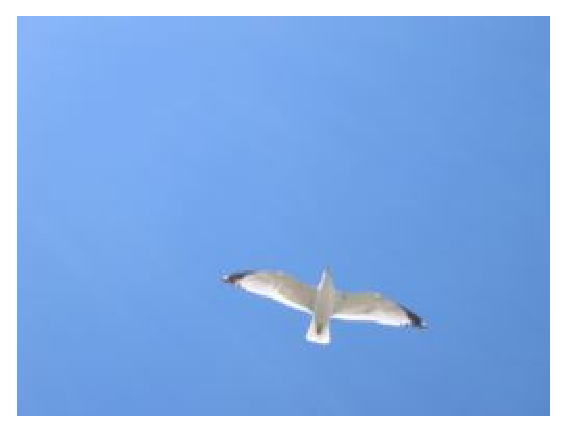
\includegraphics[width=0.4\linewidth]{seagull2.eps}
				\caption{\label{fig:seagull}}
			\end{center}
		\end{figure}
		
	\begin{itemize}
		\item ただし、コロンがついている方がよい場合は、{\tt \verb"\qUseStandardCaptions"}を入れます。
			\begin{inputbox}
				\begin{verbatim}
					\qUseStandardCaptions
				\end{verbatim}
			\end{inputbox}
		\item コロン無しに戻すためには、{\tt \verb"\qUseNoColonInCaptions"}を入れます。
			\begin{inputbox}
				\begin{verbatim}
					\qUseNoColonInCaptions
				\end{verbatim}
			\end{inputbox}
	\end{itemize}


\clearpage
\section{フォーマットの調整}
	問題の番号のフォーマットや、問題のリストの前後のスペースなどを自由に設定することができます。
	気に入った形式が決まったら、それらのコマンドを一つのファイル
	(例えば{\tt \verb"my_question_style.tex"})にまとめ、
	{\tt \verb"\input{my_question_style}"}で取り込めるようにすると楽です。
	複数人で複数の問題を作るときも、形式を決めるファイルを共有すれば便利です。
	
\subsection{印刷する領域の変更}
	印刷する領域を変更するには、いくつかの方法があります。
	\begin{itemize}
		\item {\tt \verb"\documentclass[a4j,11pt]{jarticle}"} のように"a4j"を指定する。
		\item {\tt \verb"\usepackage[a4paper]{geometry}"} のように{\tt geometry}パッケージを用いる。
		\item {\tt \verb"\usepackage[a4paper,text={17cm,25cm},centering]{geometry}"} のようにして
			印刷する領域を広げる。
	\end{itemize}
	
\subsection{ページ番号を入れない場合}
	{\tt \verb"\begin{document}"}の前に
	\begin{inputbox}
		\begin{verbatim}
			\pagestyle{empty}
		\end{verbatim}
	\end{inputbox}
	を入れます。
	
\subsection{大問と同じ行に地の文を続ける場合}
	大問と同じ行に、地の文を続ける場合は、{\tt \verb"\question{...}"}の代わりに、
	{\tt \verb"\questionNoSkip{...}"}を用います。
	\begin{inputbox}
		\begin{verbatim}
			\questionNoSkip{Q1}{次の問にすかさず答えよ。}
		\end{verbatim}
	\end{inputbox}
	
	\begin{outputbox}
	\questionNoSkip{Q1}{次の問にすかさず答えよ。}
	\end{outputbox}
	
\subsection{大問のフォーマット}
	大問の形式は、{\tt \verb"\renewcommand{\questionFormat}[1]{...}"}を用いて変えられます。
	\subsubsection{〔 〕で囲む場合}
		\begin{inputbox}
			\begin{verbatim}
				\renewcommand{\questionFormat}[1]{%
					{\Large 〔{\gt #1}〕}~%
				}
				\question{1} % 全角の数字を使ってみた
			\end{verbatim}
		\end{inputbox}
		
		\renewcommand{\questionFormat}[1]{%
			{\Large 〔{\gt #1}〕}~%
		}
		
		\begin{outputbox}
			\question{1}
		\end{outputbox}
		

	\subsubsection{四角で囲む場合}
		\begin{inputbox}
			\begin{verbatim}
				\renewcommand{\questionFormat}[1]{%
				    \framebox{\LARGE{#1}}
				}
				\question{問1}
			\end{verbatim}
		\end{inputbox}
		
		\renewcommand{\questionFormat}[1]{%
			\framebox{\LARGE{#1}}
		}
		\begin{outputbox}
			\question{問1}
		\end{outputbox}
		
	\subsubsection{少し左に寄せ、大きく、[ ]で囲む場合}
		\begin{inputbox}
			\begin{verbatim}
				\renewcommand{\questionFormat}[1]{%
				    \hspace{-3mm}\textbf{\Huge{[#1]}}
				}
				\question{1}
			\end{verbatim}
		\end{inputbox}
		\renewcommand{\questionFormat}[1]{%
			\hspace{-3mm}\textbf{\Huge{[#1]}}
		}

		\begin{outputbox}
			\question{1}
		\end{outputbox}
			
	\subsubsection{センタリングする場合}
		\begin{inputbox}
			\begin{verbatim}
				\renewcommand{\questionFormat}[1]{%
				    \begin{center}{\textbf{\LARGE{#1}}}\end{center}
				}
				\question{問題1}
			\end{verbatim}
		\end{inputbox}

		\renewcommand{\questionFormat}[1]{%
			\begin{center}{\textbf{\LARGE{#1}}}\end{center}
		}
		\begin{outputbox}
			\question{問題1}
		\end{outputbox}
			

\subsection{中問のフォーマット}
	中問の番号のフォーマットは、{\tt \verb"\renewcommand{\qpartFormat}[1]{...}"}を用いて変えられます。
	
\subsubsection{アラビア数字で}
	\begin{inputbox}
		\begin{verbatim}
			\renewcommand{\qpartFormat}[1]{%
			    \item [\textbf{\arabic{#1}}.]
			}
			\begin{qparts}
			    \qpart アラビアに行こう。
			\end{qparts}
		\end{verbatim}

	\end{inputbox}
	
	\begin{outputbox}
		\renewcommand{\qpartFormat}[1]{%
			\item [\textbf{\arabic{#1}}.]
		}
		\begin{qparts}
			\qpart アラビアに行こう。
		\end{qparts}
	\end{outputbox}
	
\subsubsection{アルファベットで大きく}
	\begin{inputbox}
		\begin{verbatim}
			\renewcommand{\qpartFormat}[1]{%
			    \item [\LARGE{\textbf{\Alph{#1}}.}]
			}
			\begin{qparts}
			    \qpart アルファベットで書いてみよう。
			\end{qparts}
		\end{verbatim}

	\end{inputbox}
	
	\begin{outputbox}
		\renewcommand{\qpartFormat}[1]{%
			\item [\LARGE{\textbf{\Alph{#1}}.}]
		}
		\begin{qparts}
			\qpart アルファベットで書いてみよう。
		\end{qparts}
	\end{outputbox}
	
\subsection{小問のprefix}
	小問は通常 {\bf (1)}, {\bf (2)}, ... という番号が付きますが、
	{\bf (E-1)}, {\bf (E-2)}, ... というように前に文字列 (prefix)をつけたい場合は、
	{\tt \verb"\begin{qlist}[E-]"} のように、{\tt [...]}をつけて({\tt \{...\}}ではない)prefixを指定します。
	\begin{inputbox}
		\begin{verbatim}
			\begin{qlist}[E-]
			    \qitem "Thunderbirds are go!"を文法的に解説せよ。
			    \qitem "I loves you, Porgy"という曲のタイトルを文法的に解説せよ。
			\end{qlist}
		\end{verbatim}
	\end{inputbox}
	
	\begin{outputbox}
			\hspace{5mm}
			\begin{minipage}{0.8\linewidth}
			\begin{qlist}[E-]
			    \qitem "Thunderbirds are go!"を文法的に解説せよ。
			    \qitem "I loves you, Porgy"という曲のタイトルを文法的に解説せよ。
			\end{qlist}
			\end{minipage}
	\end{outputbox}
	

\subsection{微小問のprefix}
	微小問は通常、小問ごとに {\bf (a)}, {\bf (b)}, ... とつけられますが、
	この前にprefixを入れたい場合は同様に{\tt qlist2}にオプションを用いてprefixを指定します。、
	例えば、prefixとして小問の番号を入れる場合は、次のようにします。
	{\tt enumi}は、小問の番号 (一番上のenumerated listの番号)を表す\LaTeX のカウンタです。
	
	\begin{inputbox}
		\begin{verbatim}
		\begin{qlist}
		    \qitem 次の物の速度を比較せよ。
		        \begin{qlist2}[\arabic{enumi}-]
		            \qitem F-16 Falcon と Millennium Falcon
		            \qitem Millennium Falconと光速
		        \end{qlist2}
		\end{qlist}
		\end{verbatim}
	\end{inputbox}
	
	\begin{outputbox}
		\begin{qlist}
		    \qitem 次の物の速度を比較せよ。
		        \begin{qlist2}[\arabic{enumi}-]
		            \qitem F-16 Falcon と Millennium Falcon
		            \qitem Millennium Falconと光速
		        \end{qlist2}
		\end{qlist}
	\end{outputbox}
	


\subsection{全体を通して(微)小問のフォーマットを変える場合}
	全ての小問のフォーマットを変える場合は{\tt \verb"\qitemFormati"}、
	微小問のフォーマットを変える場合は{\tt \verb"\qitemFormatii"}を再定義します。
	
	この方法により、問題番号に( ) がつかないようにしたり、
	問題番号を\verb"\arabicz{}" (湯川諭氏作成)を用いて、
	全角の数字にすることもできます。
	\begin{inputbox}
		\begin{verbatim}
			\renewcommand{\qitemFormati}[1]{%
			    \textbf{小問 #1\arabicz{\arabic{enumi}}}
			}
			\renewcommand{\qitemFormatii}[1]{%
			    \textbf{#1 その\arabic{enumii}}
			}
			\begin{qlist}
			    \qitem あああ(問題番号は全角)
			    \qitem いいい
			        \begin{qlist2}
			            \qitem ナノなのだ(問題番号は半角)
			            \qitem ピコなのだ
			        \end{qlist2}
			\end{qlist}
		\end{verbatim}
	\end{inputbox}
	
	\begin{outputbox}
		\hspace{5mm}
		\begin{minipage}{0.9\linewidth}
                        \renewcommand{\qitemFormati}[1]{%
                        		\textbf{小問 #1\arabicz{\arabic{enumi}}}
                        }
                        \renewcommand{\qitemFormatii}[1]{%
                        		\textbf{#1 その\arabic{enumii}}
                        }
			\begin{qlist}
				\qitem あああ(問題番号は全角)
				\qitem いいい
					\begin{qlist2}
						\qitem ナノなのだ(問題番号は半角)
						\qitem ピコなのだ
					\end{qlist2}
			\end{qlist}
		\end{minipage}
	\end{outputbox}


\subsection{中問の前のスペース}
	各中問の前のスペースは{\tt \verb"\qpartMargin"}で調整します。
	例えば5mm伸ばすには、次のようにします。
	\begin{inputbox}
		\begin{verbatim}
			\addtolength{\qpartMargin}{5mm}
		\end{verbatim}
	\end{inputbox}
	
\subsection{小問のリストの上下のスペース}
	小問のリストの固まりの上のスペースは{\tt \verb"\qlistTopMargin"}、
		下のスペースは\\{\tt \verb"\qlistBottomMargin"}で調整します。
		例えば、上のスペースを無くし、下のスペースを3mm縮めるには次のようにします。
	\begin{inputbox}
		\begin{verbatim}
			\setlength{\qlistTopMargin}{0mm}
			\addtolength{\qlistBottomMargin}{-3mm}
		\end{verbatim}
	\end{inputbox}

\subsection{微小問のリストの上下のスペース}
	微小問のリストの固まりの上のスペースは{\tt \verb"\qlistTwoTopMargin"}、
		下のスペースは\\{\tt \verb"\qlistTwoBottomMargin"}で調整します。

\clearpage
\section{Some tips}
	{\tt qexam.sty}とは関係ありませんが、問題を作るときに便利なTipsを紹介します。

\subsection{ベクトル}
	ベクトルは{\tt \verb"\vec{E}"}で$\vec{E}$のように表せます。
	太字で表すには{\tt bm}パッケージを用い、{\tt \verb"\bm{E}"}と書くと$\bm{E}$のようになります。
	\begin{inputbox}
		\begin{verbatim}
			\usepackage{bm}
			...
			\[ \bm{\nabla} \times \bm{E} = -\frac{\partial \bm{B}}{\partial t} \]
		\end{verbatim}
	\end{inputbox}
	
	\begin{outputbox}
				\[ \bm{\nabla} \times \bm{E} = -\frac{\partial \bm{B}}{\partial t} \]
	\end{outputbox}
	
\subsection{下線}
	\LaTeX 標準の{\tt \textbackslash underline}では、複数行にまたがって下線を引くことができません。
	
	{\tt udline.sty} 
	\footnote{{\tt http://homepage2.nifty.com/domae/tex/udline.html}}を用いると、
	\ul{{\tt \textbackslash ul\{...\}}で複数行の日本語への下線、
	{\tt \textbackslash Eul\{...\}}で複数行の英語への下線を引く事ができます。}
	
\subsection{PDFの図を取り込む}
	PDFの図を取り込むためには、次のようにします。
	\begin{enumerate}
		\item \LaTeX ソースファイルの頭の{\tt \textbackslash documentclass[...]{jarticle}}に例えば下のように
			\verb"dvipdfmx"を追加します。
			\begin{inputbox}
				\begin{verbatim}
					\documentclass[dvipdfmx,a4j,12pt]{jarticle}
				\end{verbatim}
			\end{inputbox}
%		\item もしPDFファイルのバージョンが1.4以上なら、Illustrator などを用いて 1.3にします。
%			PDFのバージョンは、LinuxやMac OS Xではターミナルから\\
%			{\tt \$ head foo.pdf}\\
%			とすると\\
%			{\tt \%PDF-1.3}\\
%			のように書いてあるのを見られます。
		\item もしそれでもうまくいかなければ、
			LinuxやMac OS X では、{\tt extractbb}コマンドを用いて{\tt bb, xbb} (bounding box)ファイルを作ります。
			例えば{\tt foo.pdf}なら\\
			{\tt \$ extractbb foo.pdf}\\
			を走らせ、{\tt foo.bb, foo.xbb}を作ります。
%		\item \LaTeX ソースファイルの{\tt \textbackslash usepackage\{graphicx\}}の行を次のように変えます。\\
%			\begin{inputbox}
%				\begin{verbatim}
%				\usepackage[dvipdfm]{graphicx}
%				\end{verbatim}
%			\end{inputbox}
			
	\end{enumerate}
	
\subsection{図を2つ横に並べる}
	図を2つ横に並べるには、次のように{\tt figure}環境の中に{\tt minipage}を二つ並べ、
	それぞれの中に図を取り込みます。
	\begin{inputbox}
		\begin{verbatim}
		    \begin{figure}[h]
		        \centering
		        \begin{minipage}[t]{0.45\linewidth}
		            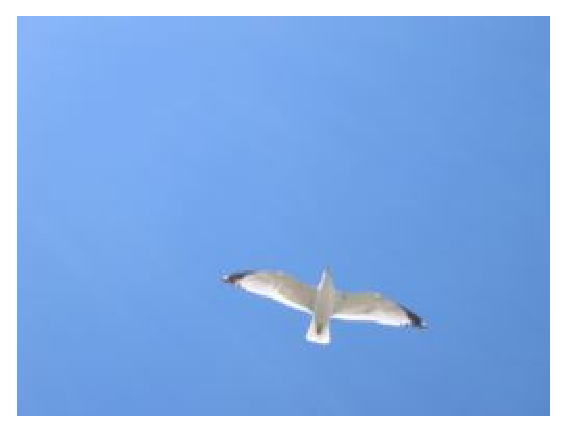
\includegraphics[width=0.95\linewidth]{seagull2.eps}
		            \caption{}
		            \label{fig:seagull}
		        \end{minipage}
		        \hspace{0.05\linewidth}
		        \begin{minipage}[t]{0.45\linewidth}
		            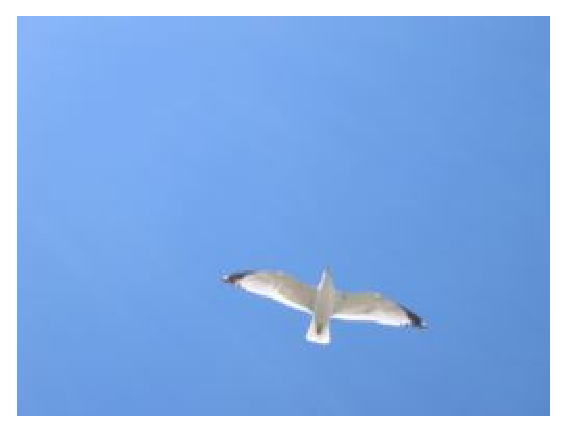
\includegraphics[width=0.95\linewidth]{seagull2.eps}
		            \caption{}
		            \label{fig:seacrow}
		        \end{minipage}
		    \end{figure}
    		\end{verbatim}
    	\end{inputbox}

		    \begin{figure}[htbp]
			\centering
		        \begin{minipage}[t]{0.45\linewidth}
		            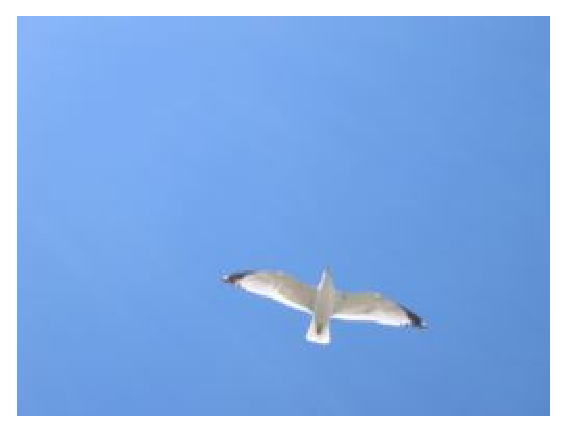
\includegraphics[width=0.95\linewidth]{seagull2.eps}
		            \caption{}
		            \label{fig:seagull}
		        \end{minipage}
		        \hspace{0.05\linewidth}
		        \begin{minipage}[t]{0.45\linewidth}
		            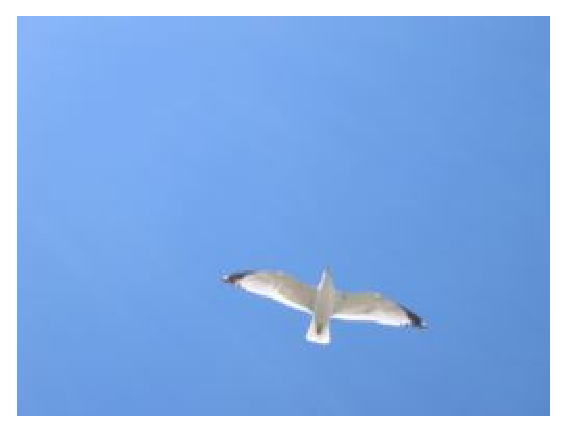
\includegraphics[width=0.95\linewidth]{seagull2.eps}
		            \caption{}
		            \label{fig:seacrow}
		        \end{minipage}
		    \end{figure}

\section{法的云々}
	\begin{itemize}
		\item {\tt qexam.sty}の配布は自由に行ってください。
			その際、この{\tt qexam\_doc.pdf}といっしょに配布してください。
		\item \begin{tiny}
			{\tt qexam.sty}を用いたことによって生じた、いかなる
			印刷ミス、出題ミス、採点ミス、悪問の発案、誤った成績判定や合否判定などについて、
			山中 卓は一切の責任を負いません。
			自己責任でお使いください。
			\end{tiny}
	\end{itemize}
\end{document}  